\documentclass[11pt]{article}
\usepackage[textwidth=18.0cm, textheight=23.0cm, top=2.0cm]{geometry}
\usepackage{pst-all}
\usepackage{amssymb}
\usepackage{tikz}
\usepackage{underscore}\begin{document}
\pagestyle{empty}


ClassName: \underline{\textbf{Class_08.2bp-9}}
\par
BinSize: \underline{\textbf{100 × 100}}
\par
ReduceSize: \underline{\textbf{100 × 100}}
\par
TypeNum: \underline{\textbf{20}}
\par
Num: \underline{\textbf{20}}
\par
OutS: \underline{\textbf{40000}}
\par
InS: \underline{\textbf{31062}}
\par
Rate: \underline{\textbf{0.777}}
\par
UB: \underline{\textbf{4}}
\par
LB0: \underline{\textbf{4}}
\par
LB: \underline{\textbf{4}}
\par
LBWithCut: \underline{\textbf{4}}
\par
NodeCut: \underline{\textbf{0}}
\par
ExtendedNodeCnt: \underline{\textbf{1}}
\par
GenNodeCnt: \underline{\textbf{1}}
\par
PrimalNode: \underline{\textbf{0}}
\par
ColumnCount: \underline{\textbf{4}}
\par
TotalCutCount: \underline{\textbf{0}}
\par
RootCutCount: \underline{\textbf{0}}
\par
LPSolverCnt: \underline{\textbf{1}}
\par
PricingSolverCnt: \underline{\textbf{0}}
\par
BranchAndBoundNum: \underline{\textbf{1}}
\par
isOpt: \underline{\textbf{true}}
\par
TimeOnInitSolution: \underline{\textbf{0.000 s}}
\par
TimeOnPrimal: \underline{\textbf{0.000 s}}
\par
TimeOnPricing: \underline{\textbf{0.000 s}}
\par
TimeOnRmp: \underline{\textbf{0.063 s}}
\par
TotalTime: \underline{\textbf{0.141 s}}
\par
\newpage


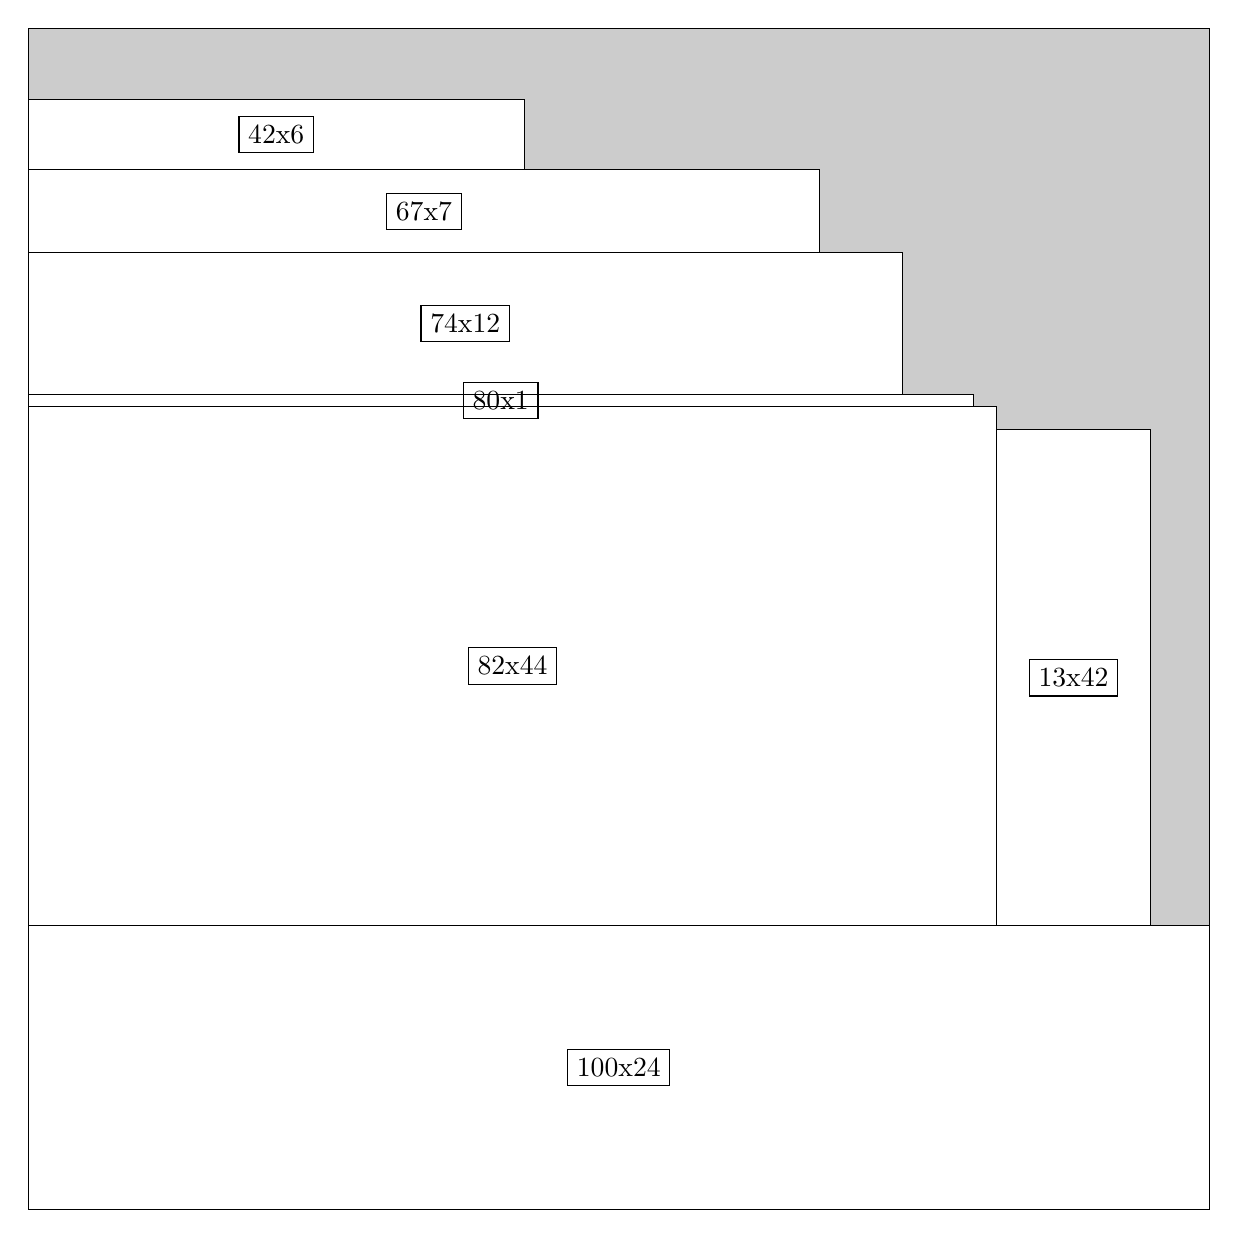
\begin{tikzpicture}[shorten >=1pt,scale=1.0,every node/.style={scale=1.0},->]
\tikzstyle{vertex}=[circle,fill=black!25,minimum size=14pt,inner sep=0pt]
\filldraw[fill=gray!40!white, draw=black] (0,0) rectangle (15.0,15.0);
\foreach \name/\x/\y/\w/\h in {82x44/0.0/3.5999999999999996/12.299999999999999/6.6,100x24/0.0/0.0/15.0/3.5999999999999996,74x12/0.0/10.35/11.1/1.7999999999999998,13x42/12.299999999999999/3.5999999999999996/1.95/6.3,67x7/0.0/12.15/10.049999999999999/1.05,42x6/0.0/13.2/6.3/0.8999999999999999,80x1/0.0/10.2/12.0/0.15}
\filldraw[fill=white!40!white, draw=black] (\x,\y) rectangle node[draw] (\name) {\name} ++(\w,\h);
\end{tikzpicture}


w =82 , h =44 , x =0 , y =24 , v =3608
\par
w =100 , h =24 , x =0 , y =0 , v =2400
\par
w =74 , h =12 , x =0 , y =69 , v =888
\par
w =13 , h =42 , x =82 , y =24 , v =546
\par
w =67 , h =7 , x =0 , y =81 , v =469
\par
w =42 , h =6 , x =0 , y =88 , v =252
\par
w =80 , h =1 , x =0 , y =68 , v =80
\par
\newpage


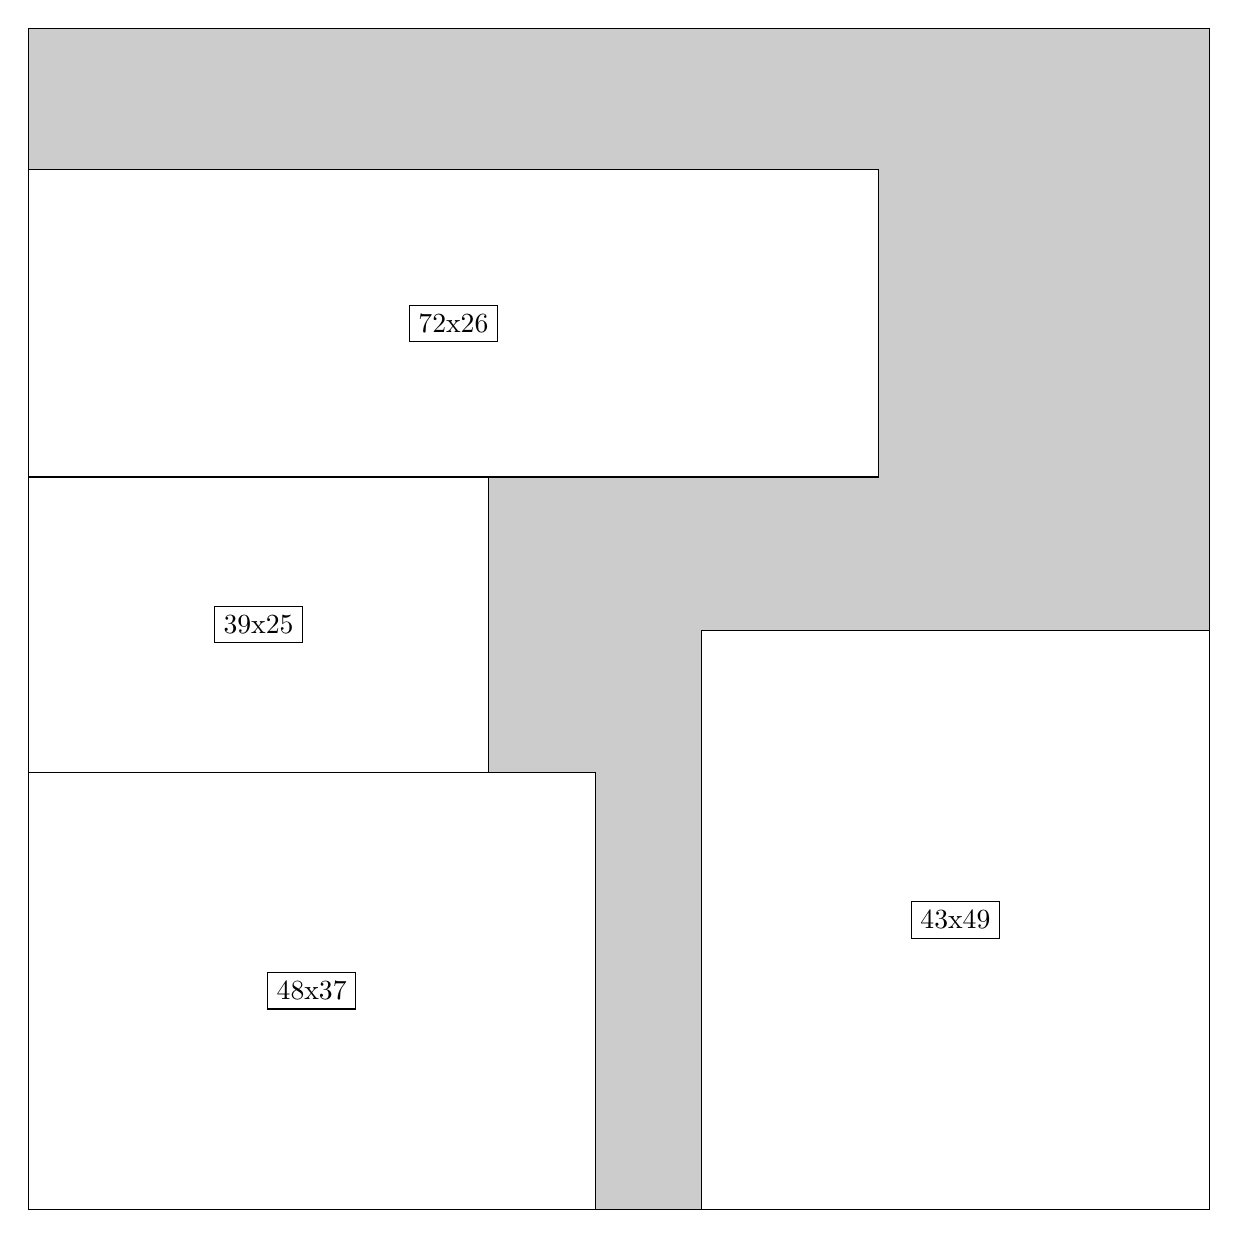
\begin{tikzpicture}[shorten >=1pt,scale=1.0,every node/.style={scale=1.0},->]
\tikzstyle{vertex}=[circle,fill=black!25,minimum size=14pt,inner sep=0pt]
\filldraw[fill=gray!40!white, draw=black] (0,0) rectangle (15.0,15.0);
\foreach \name/\x/\y/\w/\h in {72x26/0.0/9.299999999999999/10.799999999999999/3.9,48x37/0.0/0.0/7.199999999999999/5.55,43x49/8.549999999999999/0.0/6.45/7.35,39x25/0.0/5.55/5.85/3.75}
\filldraw[fill=white!40!white, draw=black] (\x,\y) rectangle node[draw] (\name) {\name} ++(\w,\h);
\end{tikzpicture}


w =72 , h =26 , x =0 , y =62 , v =1872
\par
w =48 , h =37 , x =0 , y =0 , v =1776
\par
w =43 , h =49 , x =57 , y =0 , v =2107
\par
w =39 , h =25 , x =0 , y =37 , v =975
\par
\newpage


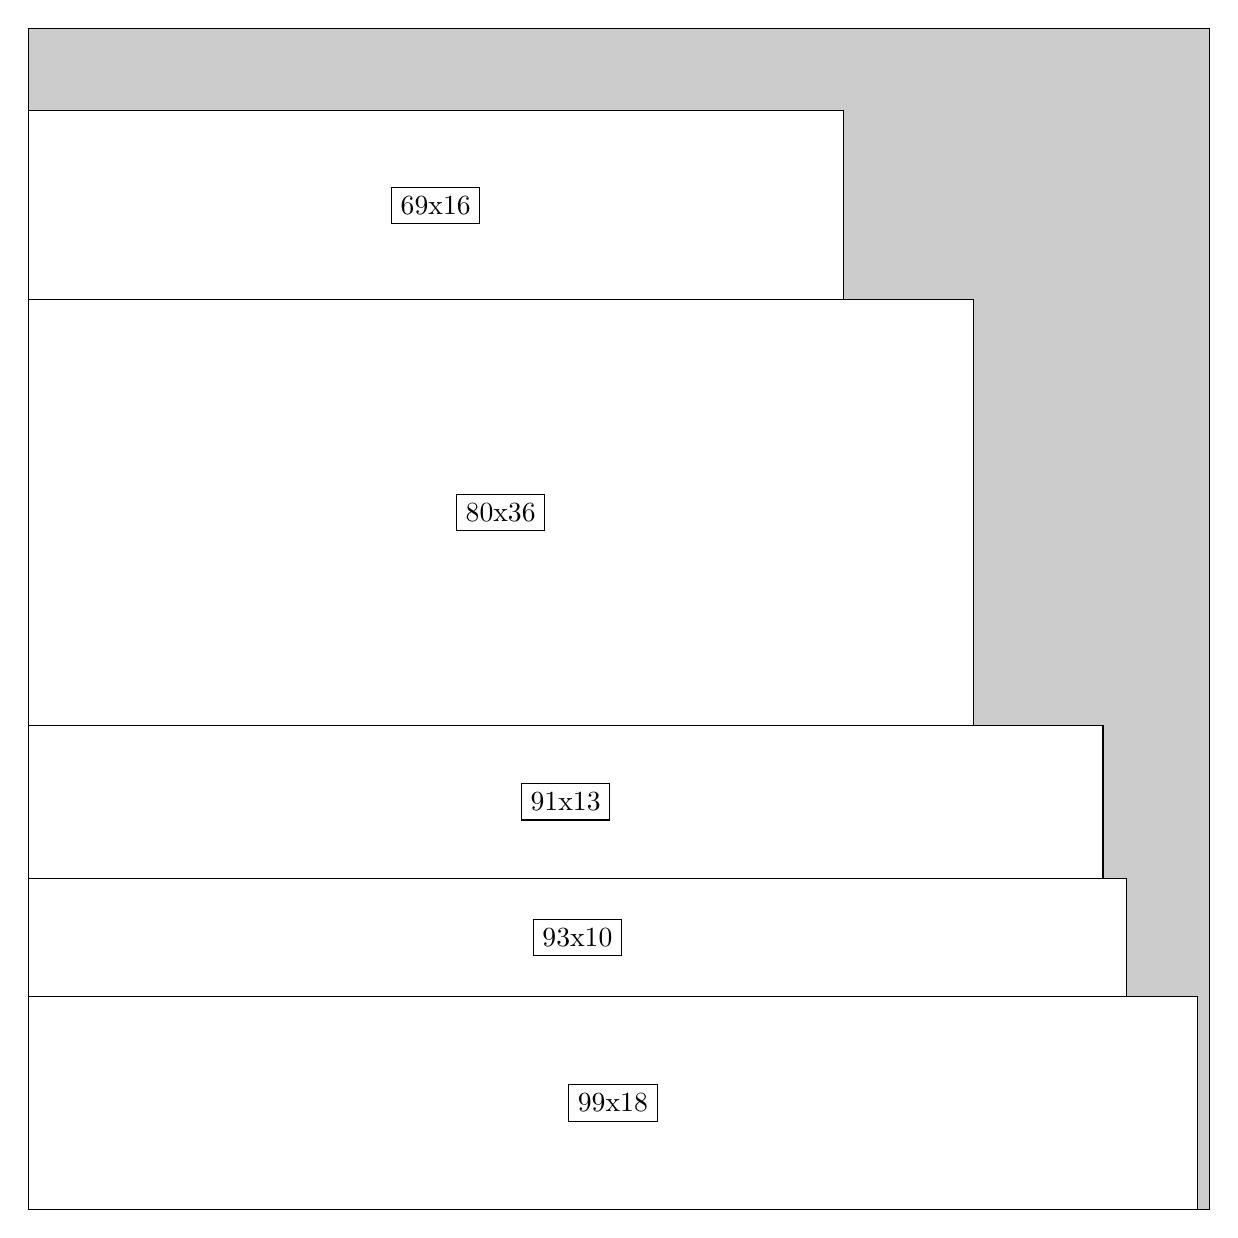
\begin{tikzpicture}[shorten >=1pt,scale=1.0,every node/.style={scale=1.0},->]
\tikzstyle{vertex}=[circle,fill=black!25,minimum size=14pt,inner sep=0pt]
\filldraw[fill=gray!40!white, draw=black] (0,0) rectangle (15.0,15.0);
\foreach \name/\x/\y/\w/\h in {80x36/0.0/6.1499999999999995/12.0/5.3999999999999995,69x16/0.0/11.549999999999999/10.35/2.4,99x18/0.0/0.0/14.85/2.6999999999999997,91x13/0.0/4.2/13.65/1.95,93x10/0.0/2.6999999999999997/13.95/1.5}
\filldraw[fill=white!40!white, draw=black] (\x,\y) rectangle node[draw] (\name) {\name} ++(\w,\h);
\end{tikzpicture}


w =80 , h =36 , x =0 , y =41 , v =2880
\par
w =69 , h =16 , x =0 , y =77 , v =1104
\par
w =99 , h =18 , x =0 , y =0 , v =1782
\par
w =91 , h =13 , x =0 , y =28 , v =1183
\par
w =93 , h =10 , x =0 , y =18 , v =930
\par
\newpage


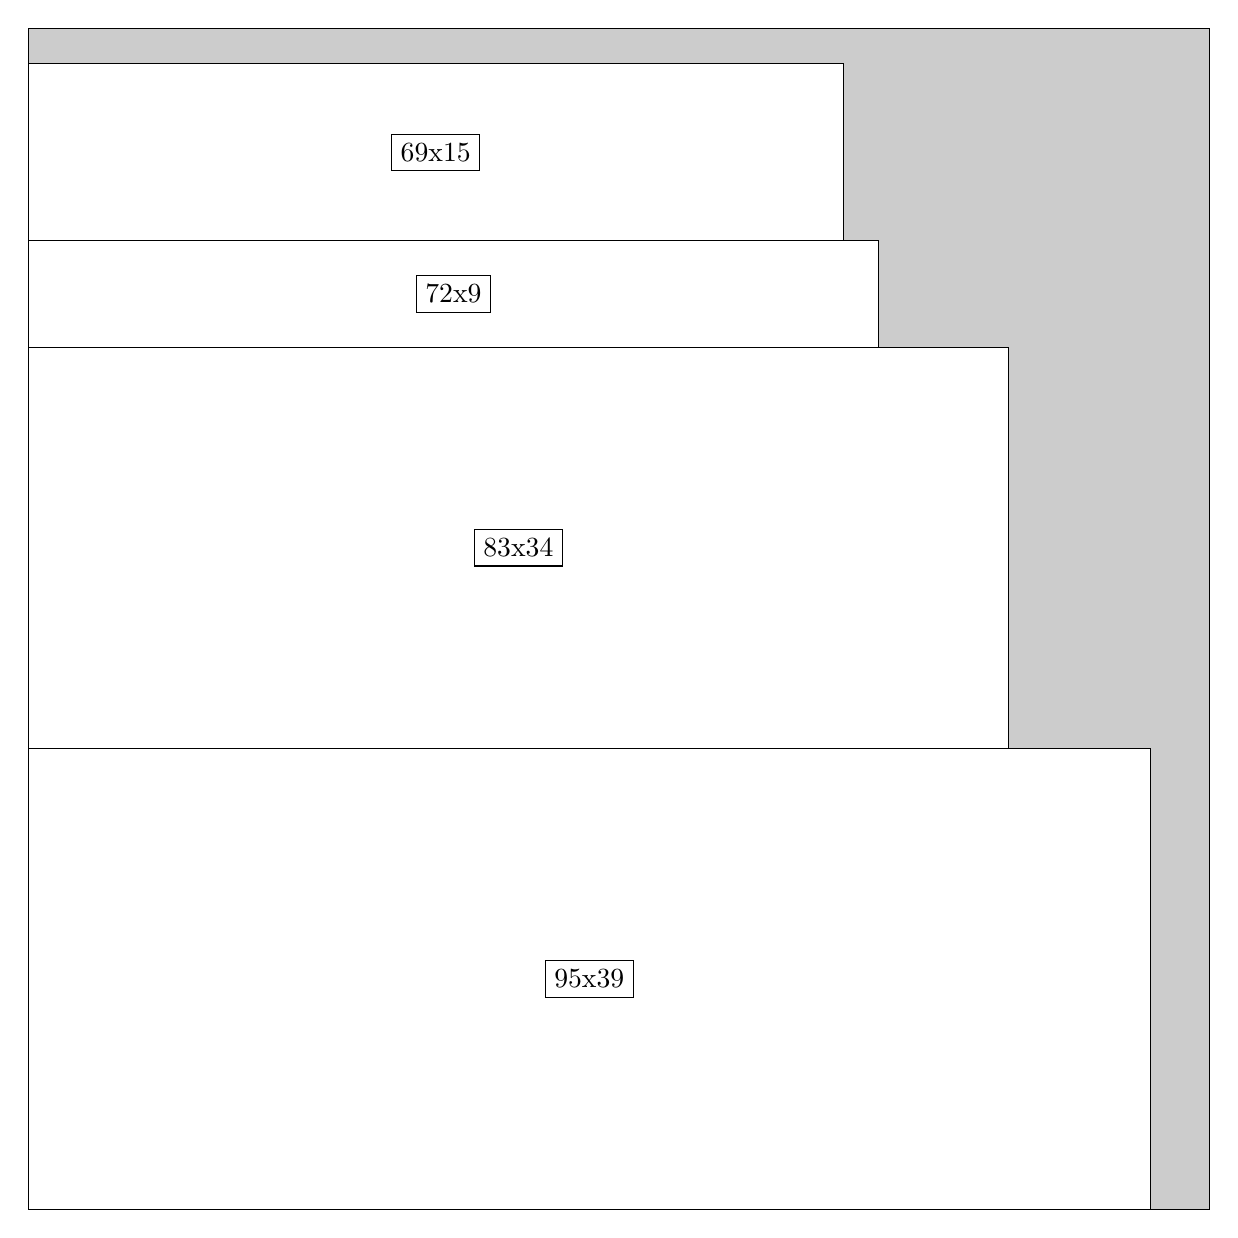
\begin{tikzpicture}[shorten >=1pt,scale=1.0,every node/.style={scale=1.0},->]
\tikzstyle{vertex}=[circle,fill=black!25,minimum size=14pt,inner sep=0pt]
\filldraw[fill=gray!40!white, draw=black] (0,0) rectangle (15.0,15.0);
\foreach \name/\x/\y/\w/\h in {95x39/0.0/0.0/14.25/5.85,83x34/0.0/5.85/12.45/5.1,69x15/0.0/12.299999999999999/10.35/2.25,72x9/0.0/10.95/10.799999999999999/1.3499999999999999}
\filldraw[fill=white!40!white, draw=black] (\x,\y) rectangle node[draw] (\name) {\name} ++(\w,\h);
\end{tikzpicture}


w =95 , h =39 , x =0 , y =0 , v =3705
\par
w =83 , h =34 , x =0 , y =39 , v =2822
\par
w =69 , h =15 , x =0 , y =82 , v =1035
\par
w =72 , h =9 , x =0 , y =73 , v =648
\par
\newpage


\end{document}